\newpage
\subsection{Μελέτη διαφορετικών Branch Predictors}
\vspace{3mm}

Στο σημείο αυτό μελετάμε την απόδοση διαφορετικών predicotrs στο σύνολο των
μετροπρογραμμάτων. Οι Predictors που συγκρίνονται είναι οι παρακάτω:

\begin{flushleft}
\begin{enumerate}
   \item Static Taken Predictor
   \item BTFNTPredictor
   \item Pentium-M
   \item Nbit-8K-4bit 
   \item LocalHistory-PHT(8K,2bit)-BHT(2K,8bit)
   \item LocalHistory-PHT(8K,2bit)-BHT(4K,4bit)
   \item GlobalHistory-PHT(16K,2bit)-BHR(5bit)
   \item GlobalHistory-PHT(8K,4bit)-BHR(5bit)
   \item GlobalHistory-PHT(8K,4bit)-BHR(10bit)
   \item GlobalHistory-PHT(16K,2bit)-BHR(10bit)
   \item Tournament(Nbit-8K-2bit, Nbit-4K-4bit)
   \item Tournament(GlobalHistory-PHT(4K,4bit)-BHR(2bit), Nbit-8K-2bit)
   \item Tournament(GlobalHistory-PHT(8K,2bit)-BHR(2bit), LocalHistory-PHT(2K,4bit)-BHT(4K,2bit))
   \item Tournament(Nbit-8K-2bit, GlobalHistory-PHT(8K,2bit)-BHR(5bit))
   \item Tournament(Nbit-2K-8bit, LocalHistory-PHT(2K,4bit)-BHT(4K,2bit))
   \item ALPHA-PREDICTOR
\end{enumerate}
\end{flushleft}

\vspace{1em}    
Ακολουθούν τα διαγράμματα που προέκυψαν και ο σχετικός σχολιασμός
τους:
\vspace{1em}    

   \begin{minipage}{\textwidth}
      \begin{center}
         \fbox{\textlatin{\textbf{\textit{403-gcc}}}}\\
         \vspace{3mm}
         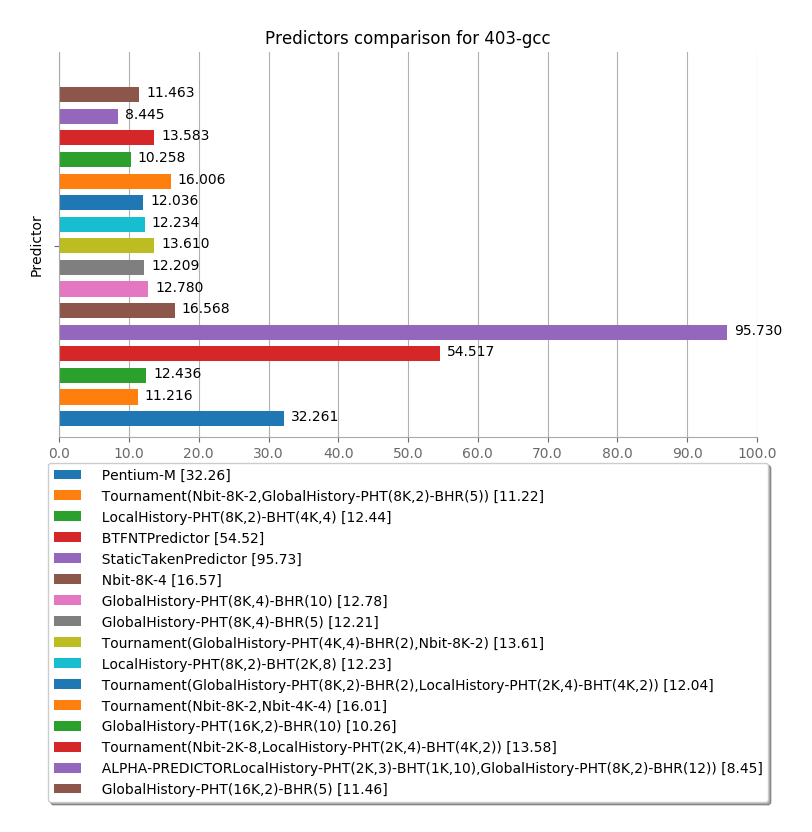
\includegraphics[width=0.9\textwidth, frame]{./graphs/4-5/403-gcc.png}
         \vspace{6mm}
      \end{center}
   \end{minipage}

   \begin{minipage}{\textwidth}
      \begin{center}
         \fbox{\textlatin{\textbf{\textit{429-mcf}}}}\\
         \vspace{3mm}
         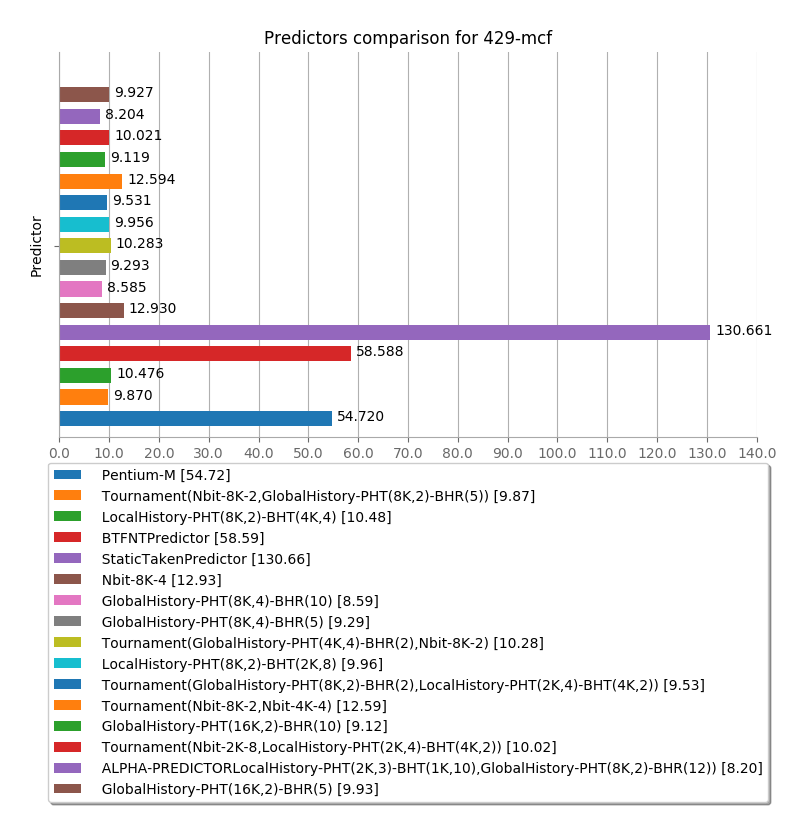
\includegraphics[width=0.9\textwidth, frame]{./graphs/4-5/429-mcf.png}
         \vspace{6mm}
      \end{center}
   \end{minipage}

   \begin{minipage}{\textwidth}
      \begin{center}
         \fbox{\textlatin{\textbf{\textit{434-zeusmp}}}}\\
         \vspace{3mm}
         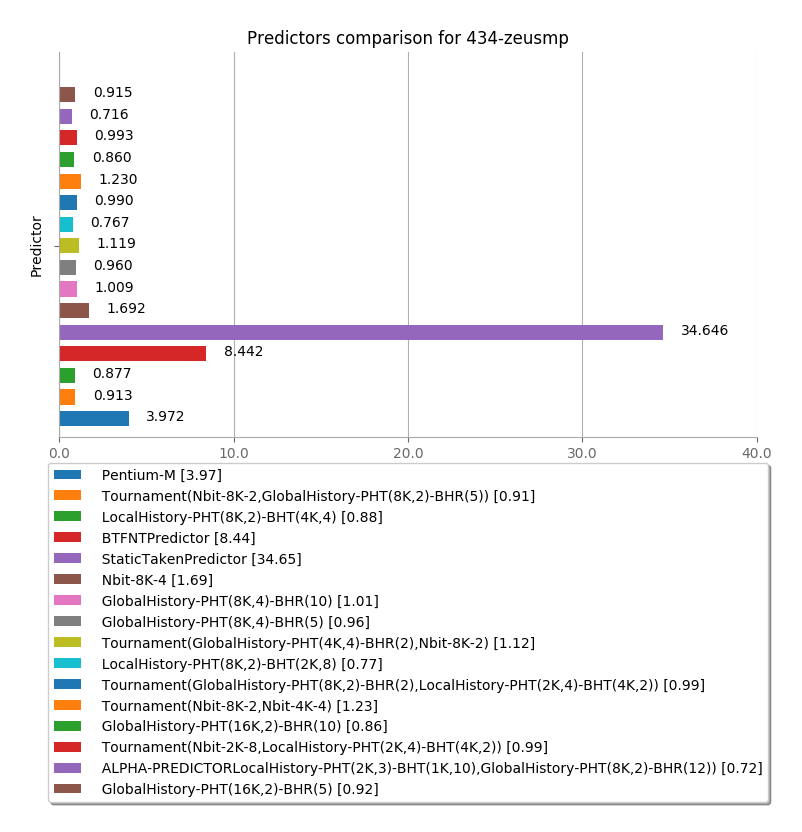
\includegraphics[width=0.9\textwidth, frame]{./graphs/4-5/434-zeusmp.png}
         \vspace{6mm}4
      \end{center}
   \end{minipage}

   \begin{minipage}{\textwidth}
      \begin{center}
         \fbox{\textlatin{\textbf{\textit{436-cactusADM}}}}\\
         \vspace{3mm}
         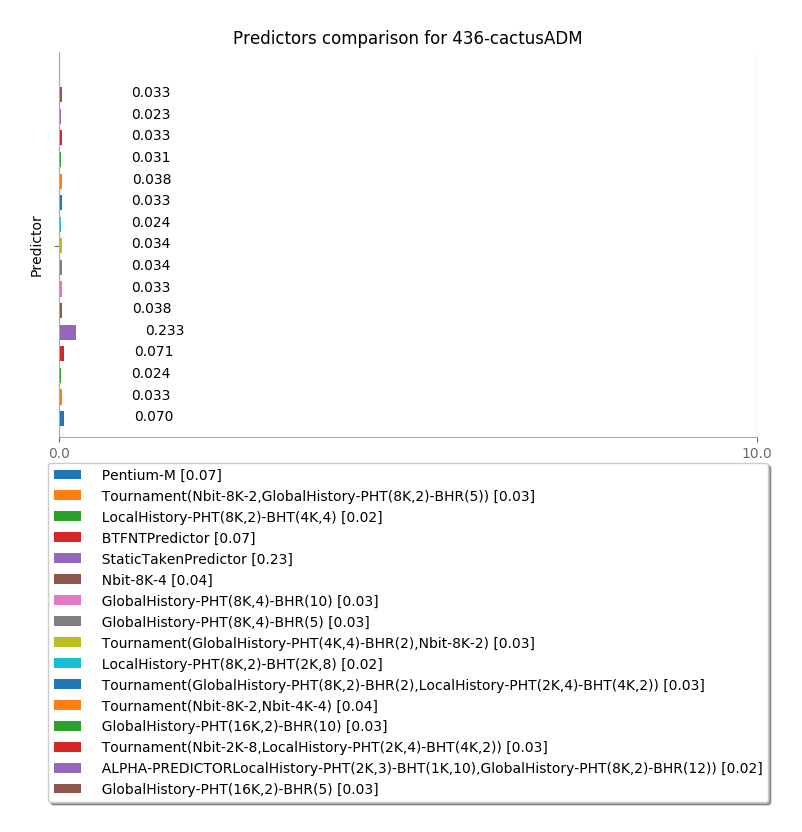
\includegraphics[width=0.9\textwidth, frame]{./graphs/4-5/436-cactusADM.png}
         \vspace{6mm}
      \end{center}
   \end{minipage}

   \begin{minipage}{\textwidth}
      \begin{center}
         \fbox{\textlatin{\textbf{\textit{445-gobmk}}}}\\
         \vspace{3mm}
         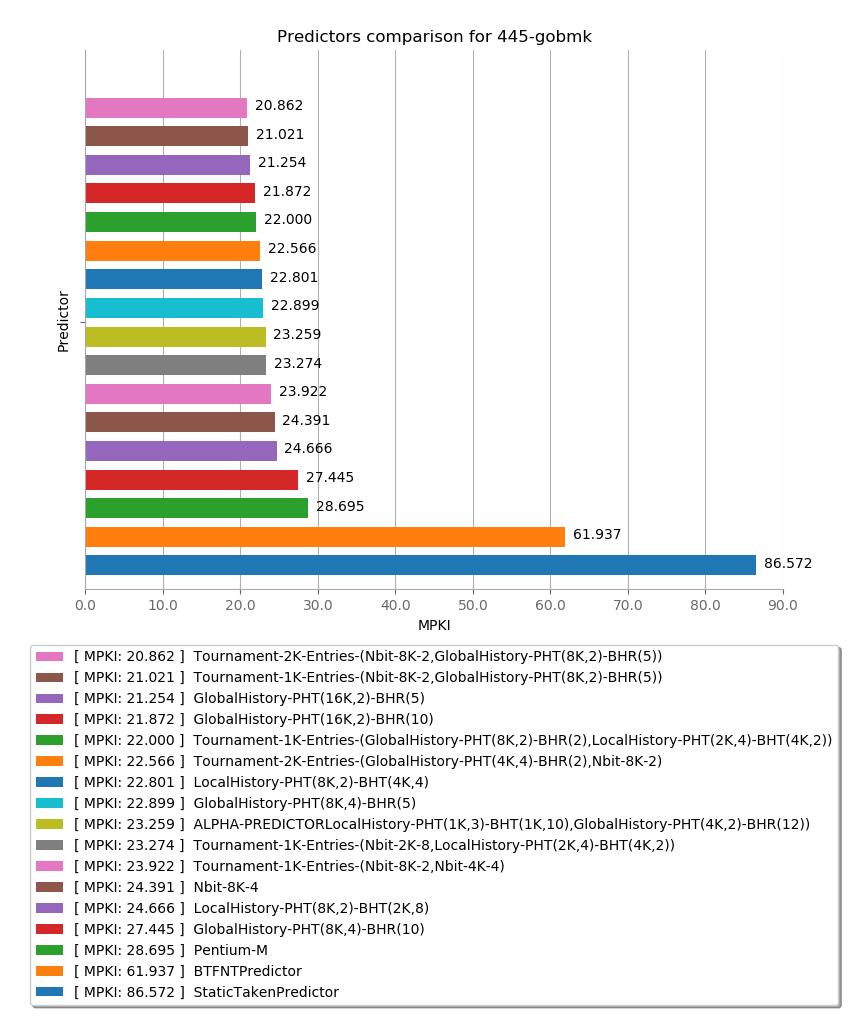
\includegraphics[width=0.9\textwidth, frame]{./graphs/4-5/445-gobmk.png}
         \vspace{6mm}
      \end{center}
   \end{minipage}

   \begin{minipage}{\textwidth}
      \begin{center}
         \fbox{\textlatin{\textbf{\textit{450-soplex}}}}\\
         \vspace{3mm}
         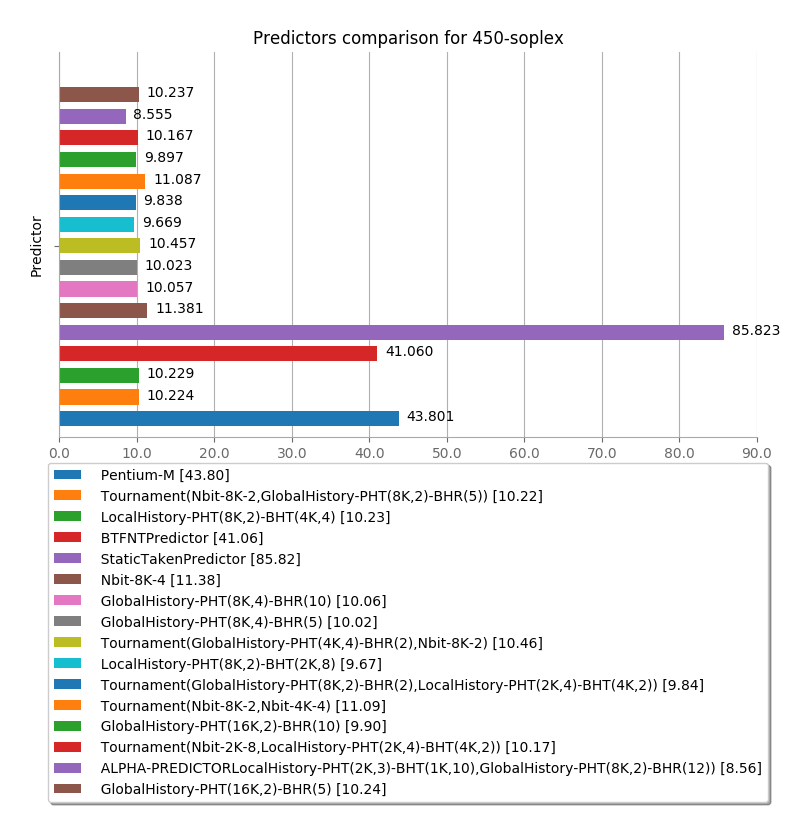
\includegraphics[width=0.9\textwidth, frame]{./graphs/4-5/450-soplex.png}
         \vspace{6mm}
      \end{center}
   \end{minipage}

   \begin{minipage}{\textwidth}
      \begin{center}
         \fbox{\textlatin{\textbf{\textit{456-hmmer}}}}\\
         \vspace{3mm}
         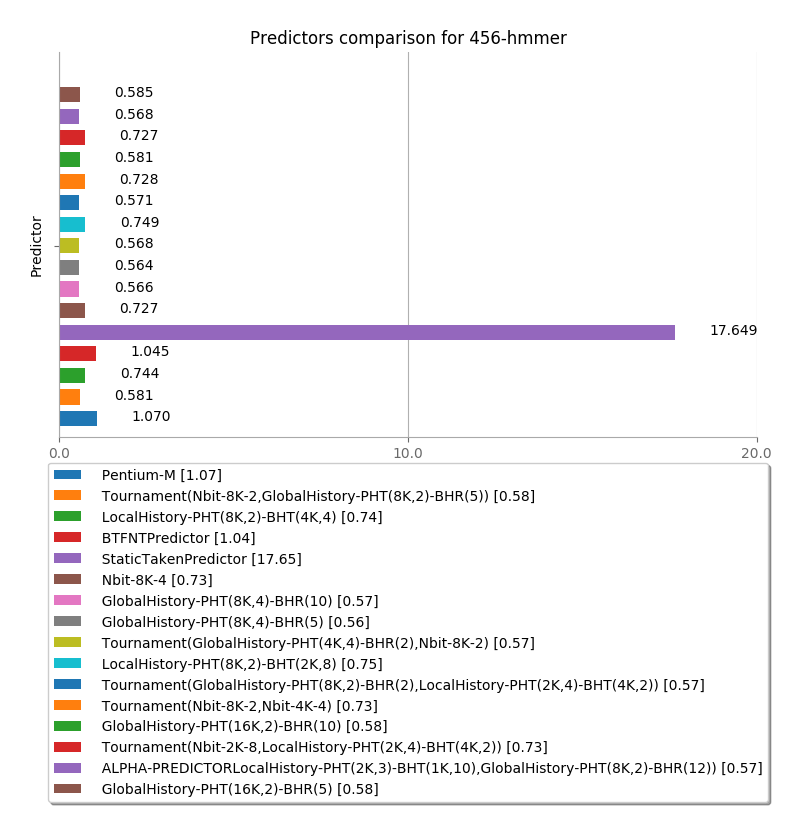
\includegraphics[width=0.9\textwidth, frame]{./graphs/4-5/456-hmmer.png}
         \vspace{6mm}
      \end{center}
   \end{minipage}

   \begin{minipage}{\textwidth}
      \begin{center}
         \fbox{\textlatin{\textbf{\textit{458-sjeng}}}}\\
         \vspace{3mm}
         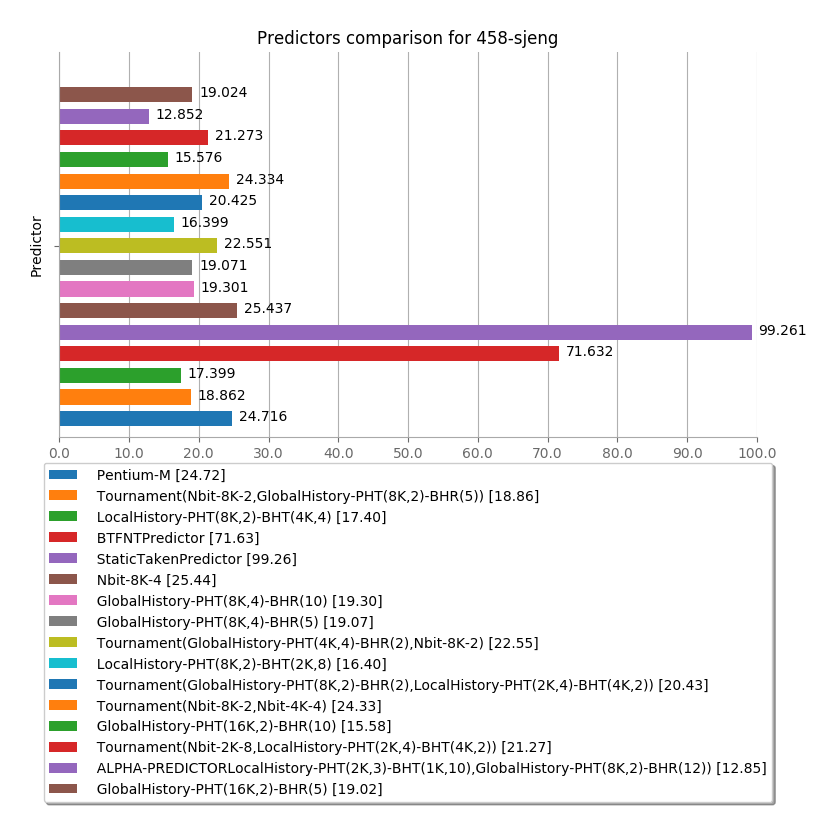
\includegraphics[width=0.9\textwidth, frame]{./graphs/4-5/458-sjeng.png}
         \vspace{6mm}
      \end{center}
   \end{minipage}

   \begin{minipage}{\textwidth}
      \begin{center}
         \fbox{\textlatin{\textbf{\textit{459-GemsFDTD}}}}\\
         \vspace{3mm}
         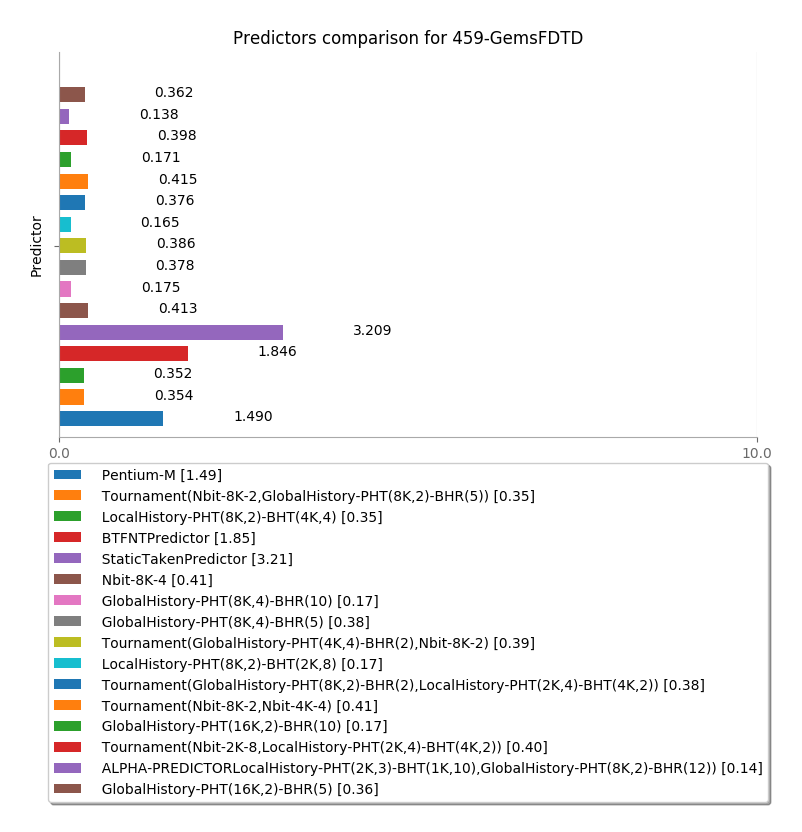
\includegraphics[width=0.9\textwidth, frame]{./graphs/4-5/459-GemsFDTD.png}
         \vspace{6mm}
      \end{center}
   \end{minipage}

   \begin{minipage}{\textwidth}
      \begin{center}
         \fbox{\textlatin{\textbf{\textit{471-omnetpp}}}}\\
         \vspace{3mm}
         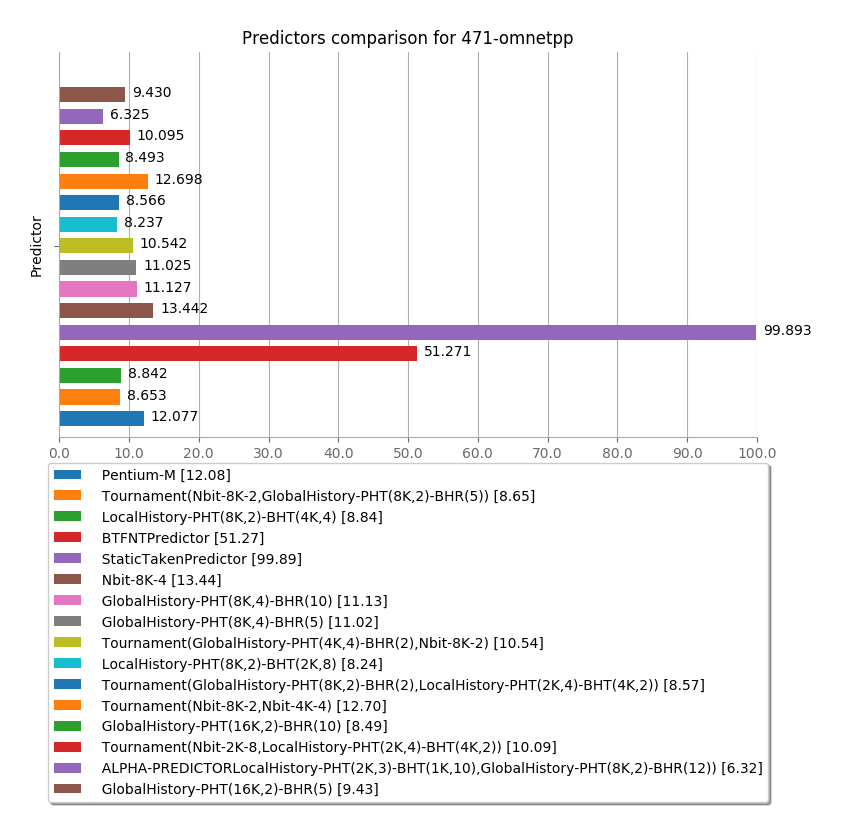
\includegraphics[width=0.9\textwidth, frame]{./graphs/4-5/471-omnetpp.png}
         \vspace{6mm}
      \end{center}
   \end{minipage}

   \begin{minipage}{\textwidth}
      \begin{center}
         \fbox{\textlatin{\textbf{\textit{473-astar}}}}\\
         \vspace{3mm}
         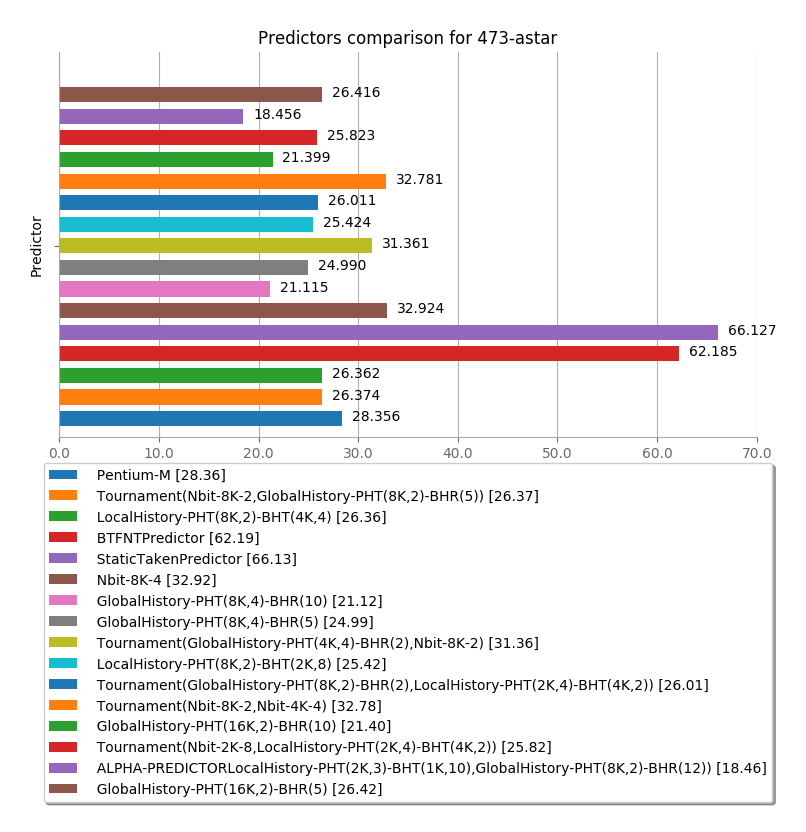
\includegraphics[width=0.9\textwidth, frame]{./graphs/4-5/473-astar.png}
         \vspace{6mm}
      \end{center}
   \end{minipage}

   \begin{minipage}{\textwidth}
      \begin{center}
         \fbox{\textlatin{\textbf{\textit{483-xalancbmk}}}}\\
         \vspace{3mm}
         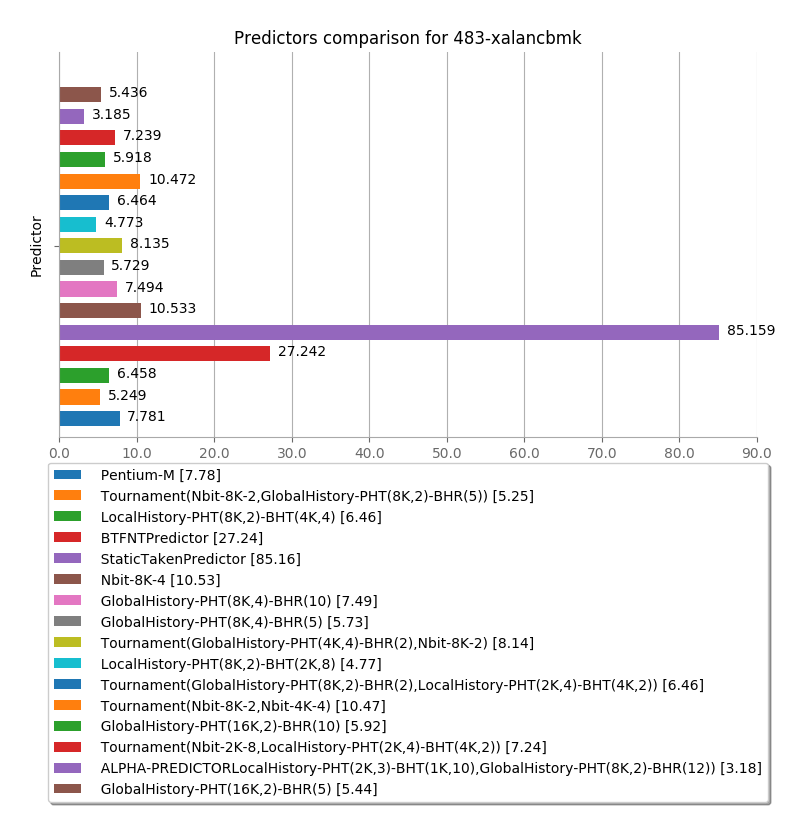
\includegraphics[width=0.9\textwidth, frame]{./graphs/4-5/483-xalancbmk.png}
         \vspace{6mm}
      \end{center}
   \end{minipage}


   \begin{minipage}{\textwidth}
      \begin{center}
         \fbox{\textlatin{\textbf{\textit{Geometric Average of MPKI}}}}\\
         \vspace{3mm}
         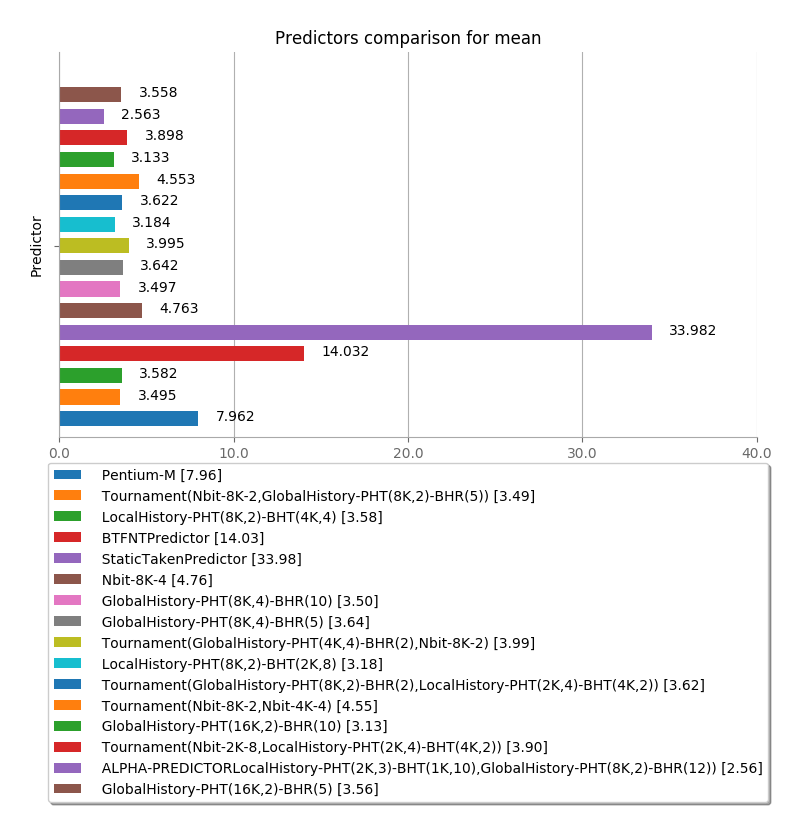
\includegraphics[width=0.9\textwidth, frame]{./graphs/4-5/mean.png}
         \vspace{6mm}
      \end{center}
   \end{minipage}

\paragraph{Συμπεράσματα-Σχόλια}
   

   Για αριθμό εγγραφών στη RAS ίσο με 1, παρατηρούμε σε σχεδόν όλα τα benchmarks
   πολύ υψηλό MPKI. Μόλις το RAS κάνει χρήση 2 εγγραφών, είναι εμφανής η
   σημαντική μείωση του MPKI. Για μεταβολή από 2 σε 4 εγγραφές, παρατηρούμε και
   πάλι σχεδόν σε όλα τα μετροπρογράμματα μείωση του MPKI, όπως είναι επιθυμητό.
   Για παραπάνω entries, τα MPKI μειώνονται μεν αλλά πλέον σχετικά λίγο, είτε
   παραμένουν σταθερά. Σε κάθε περίπτωση με την αύξηση των εγγραφών οδηγούμαστε
   σε βελτίωση της επίδοσης, ωστόσο από ένα σημείο και πέρα η περεταίρω αύξηση
   δεν έχει νόημα καθώς η επίδοση δεν βελτιώνονται δραστικά αναλογικά με την
   αύξηση του υλικού που πραγματοποιούμε. 

   Με βάση τα παραπάνω, οι επιλογή 16 ή 32 ή 64 εγγραφών είναι αρκετά καλή
   επιλογή. Αν λαμβάναμε υπ’ όψιν και το κόστος του σχετικού υλικού, τότε
   ενδεχομένως να έπρεπε να περιοριστούμε στο ελάχιστο υλικό και άρα να
   επιλέξουμε 16 εγγραφές RAS.
   
   \textbf{Συνοπτικά, καλύτερη επιλογή είναι 16 εγγραφές στην RAS}.